\chapter{相关测试}\label{chap:test}

\section{进程测试}
\subsection{程序代码}
\begin{figure}[h]
\begin{lstlisting}[caption=用户态进程创建的测试代码, label=code:testprocess]
// use user_lib::{fork, getpid, wait};
pub fn main() -> i32 {
    assert_eq!(wait(&mut 0i32), -1);
    println!("sys_wait without child process test passed!");
    println!("parent start, pid = {}!", getpid());
    let pid = fork();
    if pid == 0 {
        // child process
        println!("hello child process!");
        100
    } else {
        // parent process
        let mut exit_code: i32 = 0;
        println!("ready waiting on parent process!");
        assert_eq!(pid, wait(&mut exit_code));
        assert_eq!(exit_code, 100);
        println!("child process pid = {}, exit code = {}", pid, exit_code);
        0
    }
}
\end{lstlisting}
\end{figure}

如\autoref{code:testprocess}所示,wait在内核层是由sys\_waitpid支持的。如果当前的进程不存在子进程,则返回-1。接下来,通过fork的调用,用来创建子进程,如果成功,则会运行else部分的代码,使出子进程的退出码和pid号。 
\subsection{程序截图}

\begin{figure}[htb]
    \figureCapSet
    \centering
    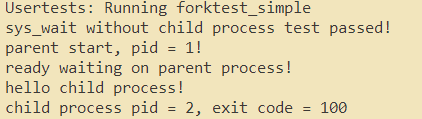
\includegraphics[scale=0.5]{figure/c5/processtestresult.png}
    \caption{进程测试的结果图}
    \label{figure:c5processtestresult}
\end{figure}

进程的测试结果如\autoref{figure:c5processtestresult}所示,遵循\autoref{code:testprocess}的执行顺序,在检测完进程是否存在子进程之后,开始创建子进程,成功创建子进程之后对子进程的相关信息pid号和退出代码。

\section{文件测试}
\subsection{程序代码}
\autoref{code:testfile}是一个用户态的文件读写的例子,代码尝试将”Hello, world!”写入filea的文件中,通过open函数, CREATE和WRONLY句柄,实现对filea文件的创建和写入。在文件打开成功之后,通过write函数将字符信息写入文件。然后,再通过open函数,RDONLY句柄将文件filea中的内容读出。两次open的操作之后都需要使用close函数关闭文件句柄,保证内存空间可以正确被释放。最后对比两者的长度,测试文件是否能正确读写。
\begin{figure}[h]
\begin{lstlisting}[caption=用户态文件读写的测试代码, label=code:testfile]
// use user_lib::{close, open, read, write, OpenFlags};
pub fn main() -> i32 {
    let test_str = "Hello, world!";
    let filea = "filea\0";
    let fd = open(filea, OpenFlags::CREATE | OpenFlags::WRONLY);
    assert!(fd > 0);
    let fd = fd as usize;
    write(fd, test_str.as_bytes());
    close(fd);

    let fd = open(filea, OpenFlags::RDONLY);
    assert!(fd > 0);
    let fd = fd as usize;
    let mut buffer = [0u8; 100];
    let read_len = read(fd, &mut buffer) as usize;
    close(fd);

    assert_eq!(test_str, core::str::from_utf8(&buffer[..read_len]).unwrap(),);
    println!("file_test passed!");
    0
}
\end{lstlisting}
\end{figure}

\autoref{code:testcat}是一个十分简化的类似于Linux中的cat函数,只是代码十分简单,类似于\autoref{code:testfile}的文件读取逻辑,在接收来自命令行的文件名后,尝试读取该文件,并通过print函数将文件信息输出到控制台。
\begin{figure}[h]
\begin{lstlisting}[caption=用户态小程序cat, label=code:testcat]
// use user_lib::{close, open, read, write, OpenFlags};
pub fn main() -> i32 {
    let test_str = "Hello, world!";
    let filea = "filea\0";
    let fd = open(filea, OpenFlags::CREATE | OpenFlags::WRONLY);
    assert!(fd > 0);
    let fd = fd as usize;
    write(fd, test_str.as_bytes());
    close(fd);

    let fd = open(filea, OpenFlags::RDONLY);
    assert!(fd > 0);
    let fd = fd as usize;
    let mut buffer = [0u8; 100];
    let read_len = read(fd, &mut buffer) as usize;
    close(fd);

    assert_eq!(test_str, core::str::from_utf8(&buffer[..read_len]).unwrap(),);
    println!("file_test passed!");
    0
}
\end{lstlisting}
\end{figure}

\subsection{程序截图}
\begin{figure}[htb]
    \figureCapSet
    \centering
    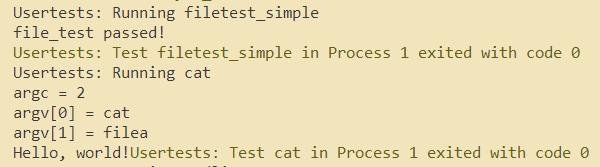
\includegraphics[scale=0.5]{figure/c5/filetestresult.png}
    \caption{文件测试的结果图}
    \label{figure:c5filetestresult}
\end{figure}
如\autoref{figure:c5filetestresult}所示,在文件测试,即file\_test成功之后,当前运行目录下会创建一个filea的文件,通过cat的小程序,读出filea中的内容。
\section{异步测试}
\subsection{程序代码}
\autoref{code:testkernelasync}是内核中测试的异步任务,在初始化内核的全局调度器之后,通过一个循环向内核的调度器添加20个打印”Hello world!”的任务。最后,内核的调度器通过run\_until\_idle异步执行20个异步的任务。

\begin{figure}[h]
\begin{lstlisting}[caption=内核异步任务测试代码, label=code:testkernelasync]
pub fn init() {
    let executor = crate::task::async_task::woke::Executor::default();

    for _ in 1..20 {
        executor.spawn(async { println!("[kernel async] Hello world!") });
    }

    executor.run_until_idle();
}
\end{lstlisting}
\end{figure}

为了能和内核的异步任务有所区别,用户态尝试通过异步来对斐波那契数列进行求值。如\autoref{code:testfibonacci}所示,FibonacciFuture记录了predecessor, successor, index,和count,分别代表了数列中当前状态值的前驱值,后继值,当前的状态标记和要求的值。斐波那契数列的计算的状态只有两个一个是完成的Ready,另一则是Pending的阻塞状态。Ready态下斐波那契数列的计算才算完成,在Pending的状态在每次状态转化都会进行数列的计算,及相应值状态升级。

\begin{figure}[h]
\begin{lstlisting}[caption=异步计算斐波那契数列, label=code:testfibonacci]
struct FibonacciFuture {
    predecessor: usize,
    successor: usize,
    index: usize,
    count: usize,
}

impl FibonacciFuture {
    fn new(count: usize) -> FibonacciFuture {
        FibonacciFuture {
            predecessor: 0,
            successor: 1,
            index: 0,
            count,
        }
    }
}

impl Future for FibonacciFuture {
    type Output = usize;
    fn poll(mut self: Pin<&mut Self>, cx: &mut Context<'_>) -> Poll<Self::Output> {
        if self.index == self.count {
            println!("[user async]\x1b[7m\x1b[31m[Fib Record]\x1b[0m\x1b[27m\x1b[0mFibonacci {} result: {}", self.count, self.predecessor);
            Poll::Ready(self.predecessor)
        } else {
            let tmp = self.predecessor;
            self.predecessor += self.successor;
            self.successor = tmp;
            self.index += 1;
            println!("[user async]\x1b[7m\x1b[96m[Fib Record]\x1b[0m\x1b[27m\x1b[0mFibonacci {}; index = {}, predecessor = {}, successor = {}", self.count, self.index, self.predecessor, self.successor);
            cx.waker().wake_by_ref();
            Poll::Pending
        }
    }
}
\end{lstlisting}
\end{figure}
为了能和内核的异步任务有所区别,用户态尝试通过异步来对斐波那契数列进行求值。如\autoref{code:testfibonacci}所示,FibonacciFuture记录了predecessor, successor, index,和count,分别代表了数列中当前状态值的前驱值,后继值,当前的状态标记和要求的值。斐波那契数列的计算的状态只有两个一个是完成的Ready,另一则是Pending的阻塞状态。Ready态下斐波那契数列的计算才算完成,在Pending的状态在每次状态转化都会进行数列的计算,及相应值状态升级。


\begin{figure}[h]
\begin{lstlisting}[caption=用户异步任务测试代码, label=code:testuserasync]
fn main() -> i32 {
    let executor = Executor::default();
    executor.spawn(async {
        let i = 50;
        let ans = FibonacciFuture::new(i).await;
        println!("[user space] Fibonacci[{}] = {}", i, ans);
    });
    executor.spawn(async {
        let i = 11;
        let ans = FibonacciFuture::new(i).await;
        println!("[user space] Fibonacci[{}] = {}", i, ans);
    });
    executor.spawn(async {
        let i = 1;
        let ans = FibonacciFuture::new(i).await;
        println!("[user space] Fibonacci[{}] = {}", i, ans);
    });
    executor.run_until_idle();
    0
}
\end{lstlisting}
\end{figure}
如\autoref{code:testuserasync}所示,与内核的异步执行逻辑类似。用户的异步任务。在获取调度器之后,分别添加计算第50位,第11位和第1位斐波那契数值的工作。然后交由调度器轮询执行任务。

\subsection{程序截图}
如\autoref{figure:c5kernelasynctestresult},遵循\autoref{code:testkernelasync}的执行逻辑,内核的异步任务可以得到正确的执行,符合设计的预期。

\begin{figure}[htb]
    \figureCapSet
    \centering
    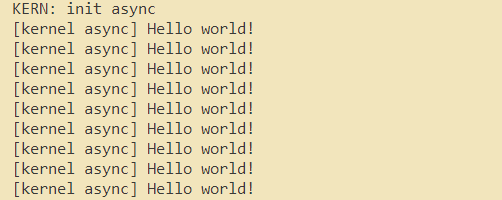
\includegraphics[scale=0.5]{figure/c5/kernelasynctestresult.png}
    \caption{内核异步测试的结果图}
    \label{figure:c5kernelasynctestresult}
\end{figure}
\begin{figure}[htb]
    \figureCapSet
    \centering
    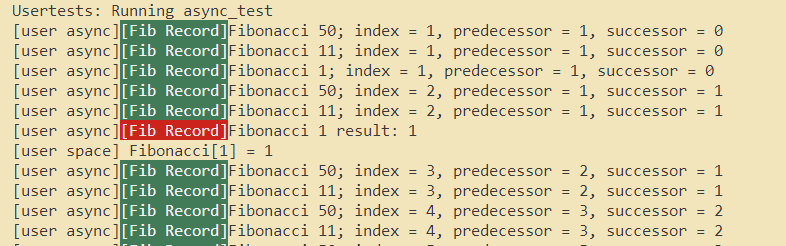
\includegraphics[scale=0.5]{figure/c5/userasynctestresult.png}
    \caption{用户态异步测试的结果图}
    \label{figure:c5userasynctestresult}
\end{figure}
\autoref{figure:c5userasynctestresult}显示了用户态的异步任务执行结果的部分截图。很明显计算斐波那契数列的第50个值比起计算第11个和第1个,所需要的语句执行频次会更多。试想一下,如果在同步的环境下,计算过于密集的计算,会占用大量的时间,这对于相对稀疏的计算是非常不公平的。如果在需求相似时,短作业的长时间等待是非常不合理的。由此,异步的提出是十分有意义的,在异步的执行器第一次轮询的时候,计算50,11和1的任务都会被掉起,而1的计算只需1状态的两次转换依次计算的Pending和依次计算的完成Ready即可,在异步轮询的第二次1的计算就完成了,此时短作业并没有因长作业而被阻塞,在软件效率上有了比较大的提升,由此证明异步的设计和开发是十分有必要的。